\subsection{供电电路测试}
\begin{table}[H]
\centering
\caption{供电测试结果}
\begin{tabular}{L{.7\textwidth}C{.2\textwidth}}
\toprule
检测项目 & 检测结果\\
\midrule
电源空载时的输出电压:  & 5.100V \\
插上电源后D3状态(亮/灭):     & 亮    \\
插上电源后,标注5V处(J1的3脚)的电压: & 5.102V\\
\bottomrule
\end{tabular}
\end{table}
再最开始通上电后,LED灯没有正常亮起,经调试发现LED灯是坏的。借助吸锡器将LED取下后更换新的重试,发现结果正常。
\begin{figure}[H]
\centering
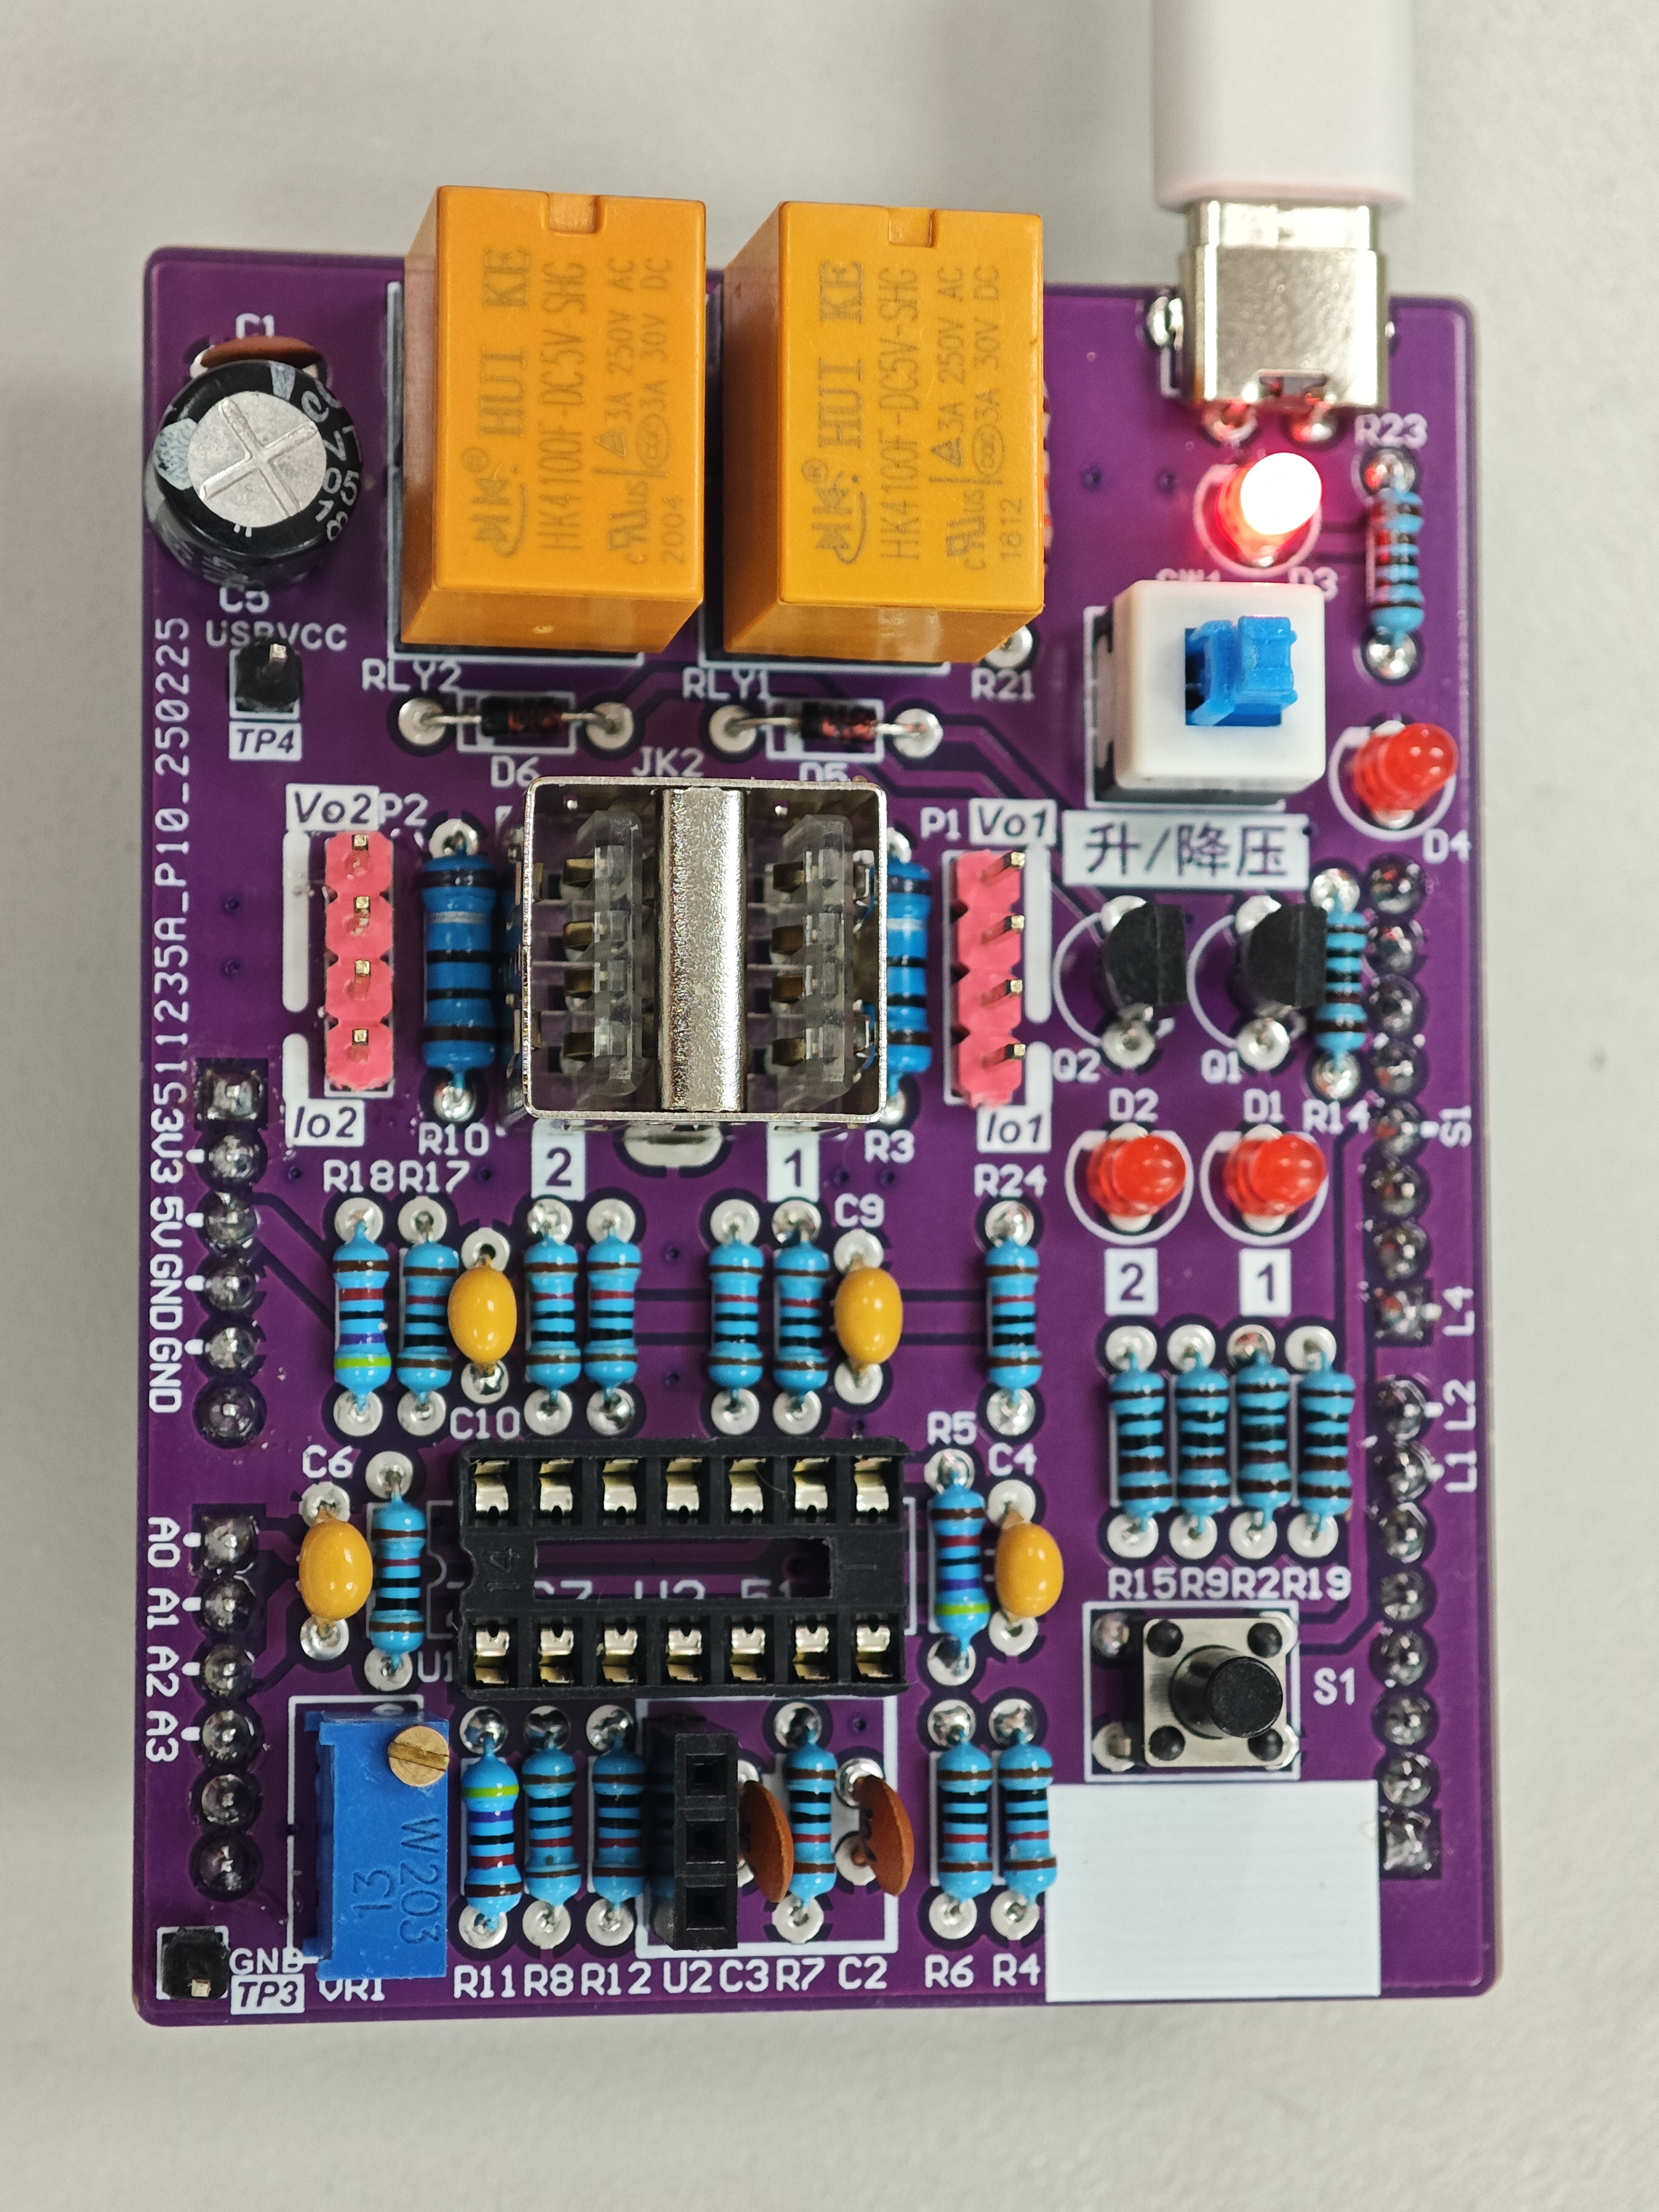
\includegraphics[width=.3\textwidth]{./figures/插座/通电.jpg}
\includegraphics[width=.3\textwidth]{./figures/插座/通电测量.jpg}
\caption{通电测量过程}
\end{figure}
\subsection{USB插座供电控制电路测试}
\textbf{USB供电通路的信号路径}:引脚 IO7 通过高/低电平(即+5V/0V),可控制三极管 Q1 的导通/截止,从而决定继电器 RLY2 的
通断,最终决定 USB 供电插座 JK2 上的 USB2 口是否有 5V(即 USBVCC)电源输出。供电电流将从
USB2 口的 VCC 引脚流出,经过外接用电器,从 USB2 口的 GND 流回。
\begin{table}[H]
\centering
\caption{USB插座供电控制电路测试结果}
\begin{tabular}{L{.4\textwidth}L{.4\textwidth}}
    \toprule
检测项目  & 检测结果 \\
\midrule
以杜邦线连接标注L1处至标注5V,观察到的现象:   & D1\underline{亮},继电器RLY1\underline{吸合},USB供电插座1的供电电压\underline{5.088V}。 \\
以杜邦线连接标注L1处至标注GND,观察到的现象: &    D1\underline{灭},继电器RLY1\underline{断开},USB供电插座1的供电电压\underline{0V}。\\
以杜邦线连接标注L2处至标注5V,观察到的现象:  & D2\underline{亮},继电器RLY2\underline{吸合},USB供电插座2的供电电压\underline{5.087V}。 \\
以杜邦线连接标注L2处至标注GND,观察到的现象:  &  D2\underline{灭},继电器RLY2\underline{断开},USB供电插座2的供电电压\underline{0V}。\\
\bottomrule
\end{tabular}
\end{table}
\begin{figure}[H]
  \centering
  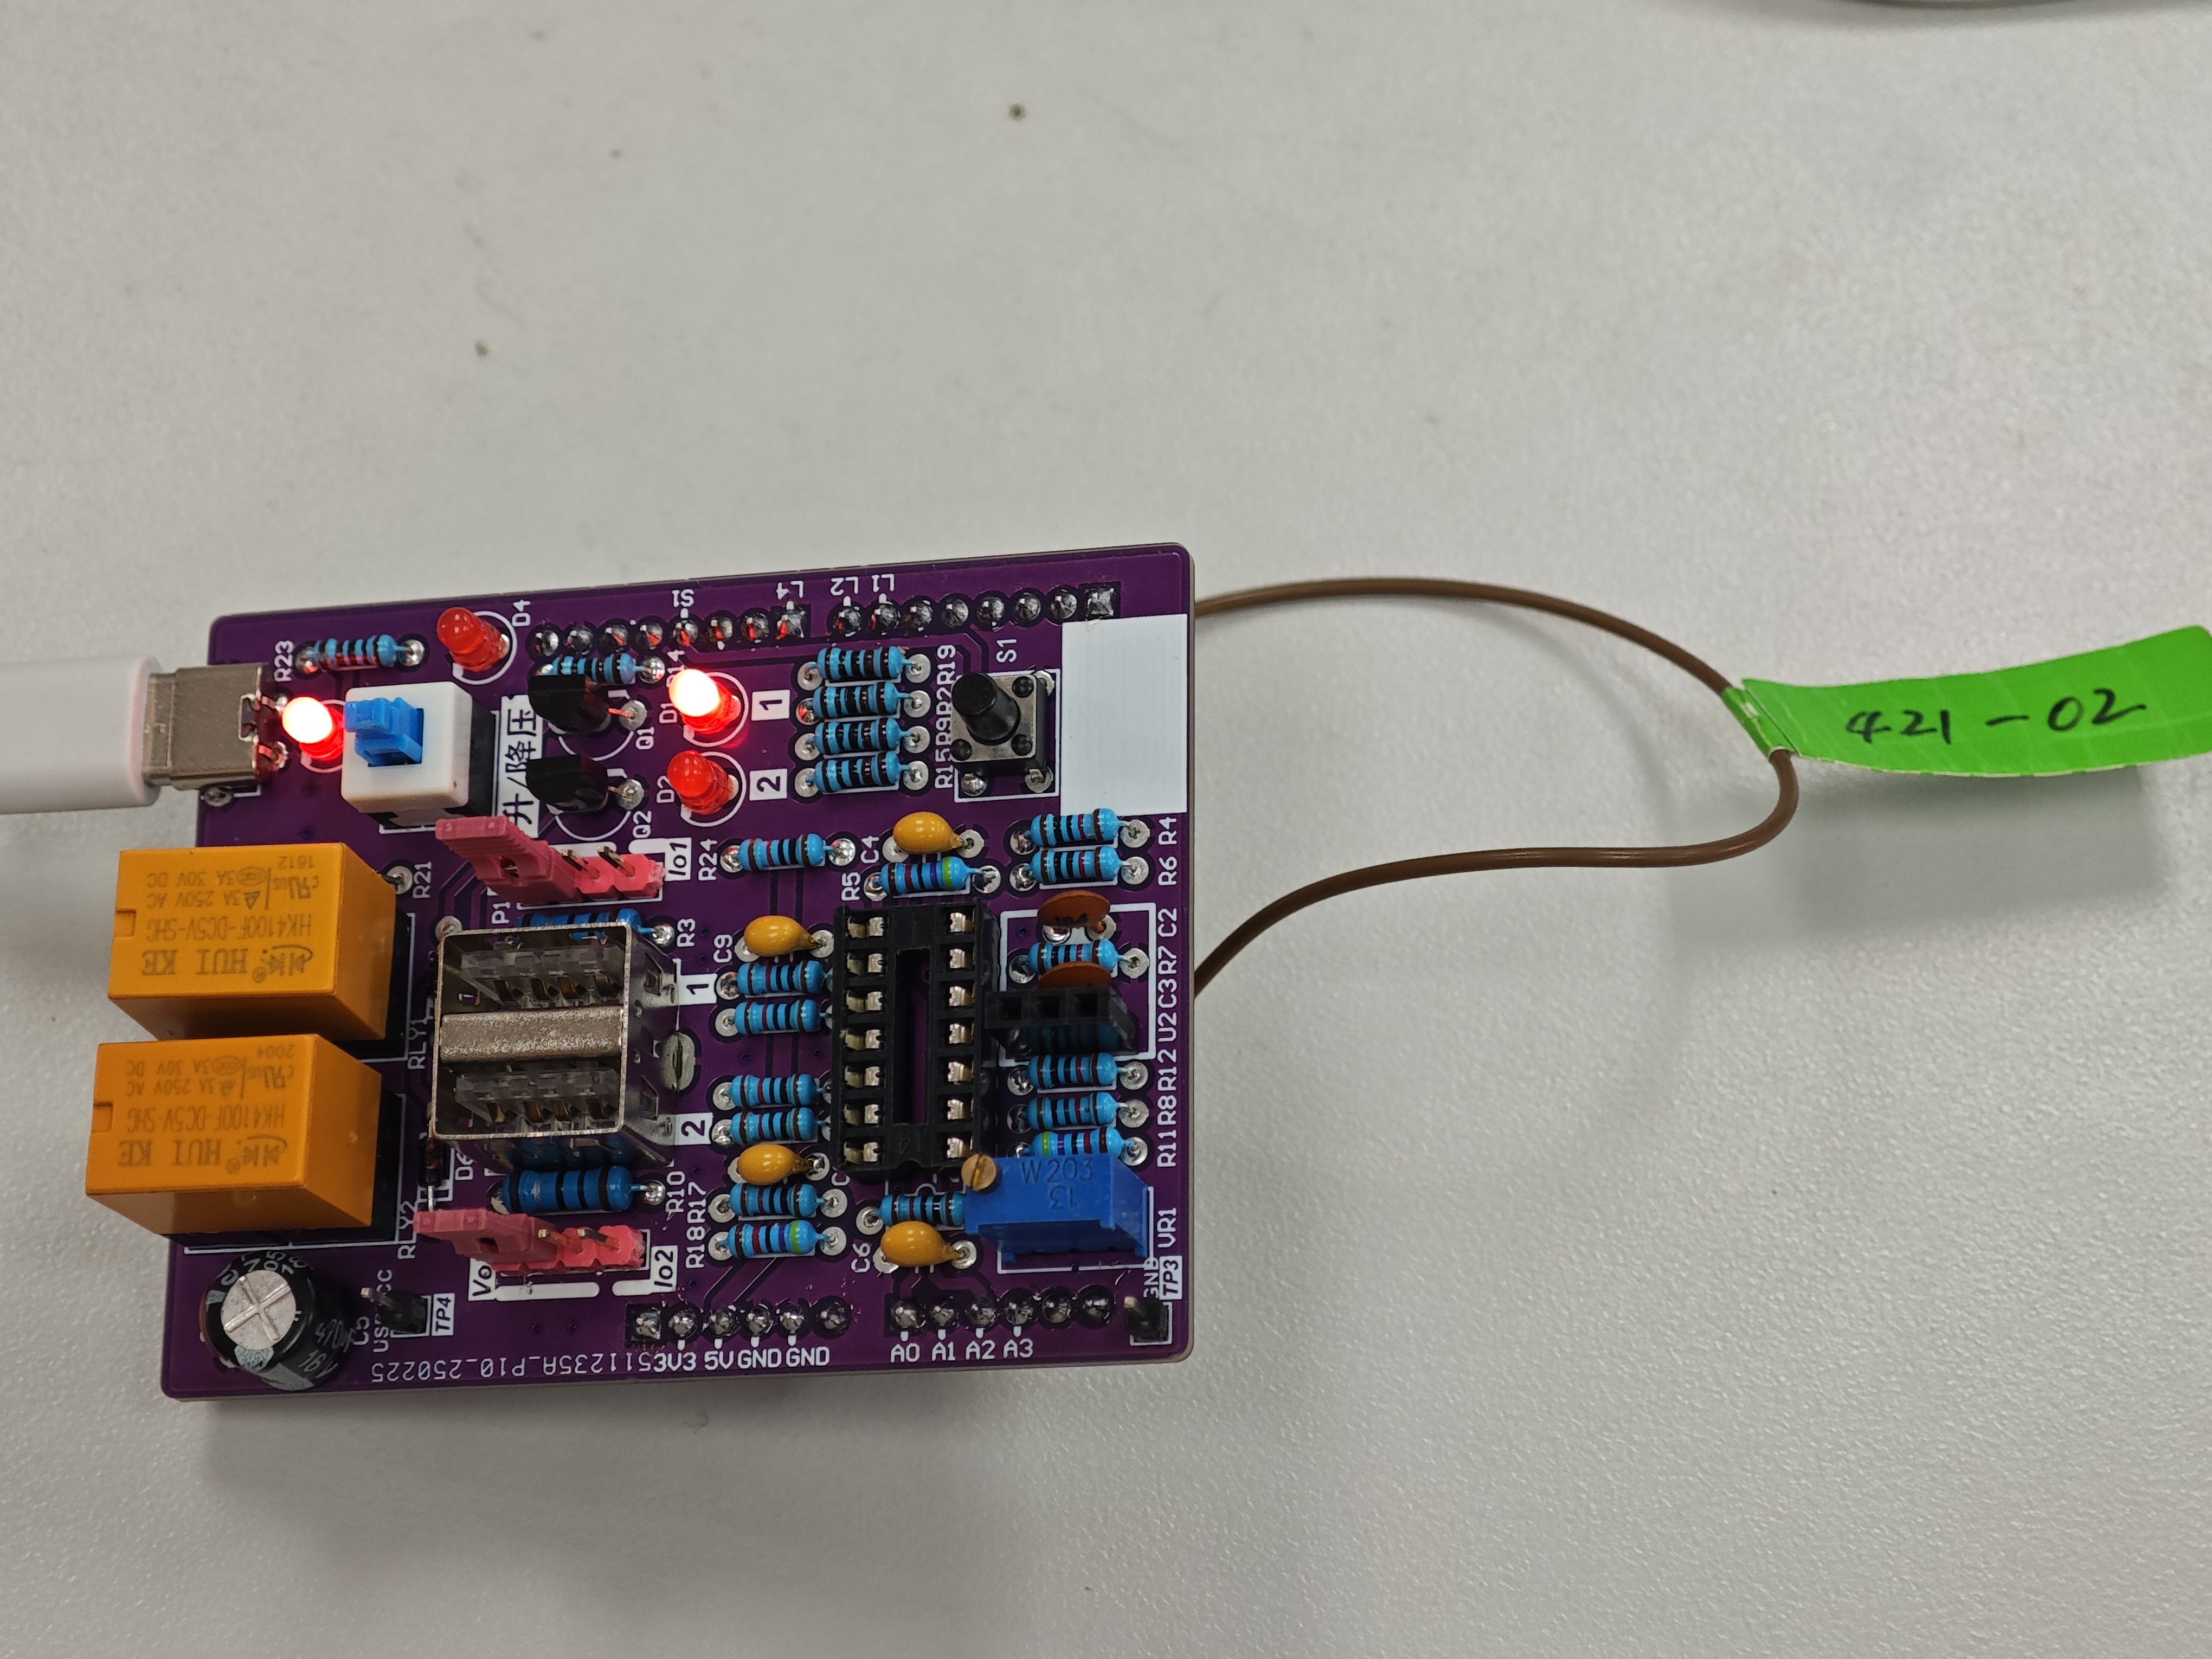
\includegraphics[width=.3\textwidth]{./figures/插座/usb1供电.jpg}
  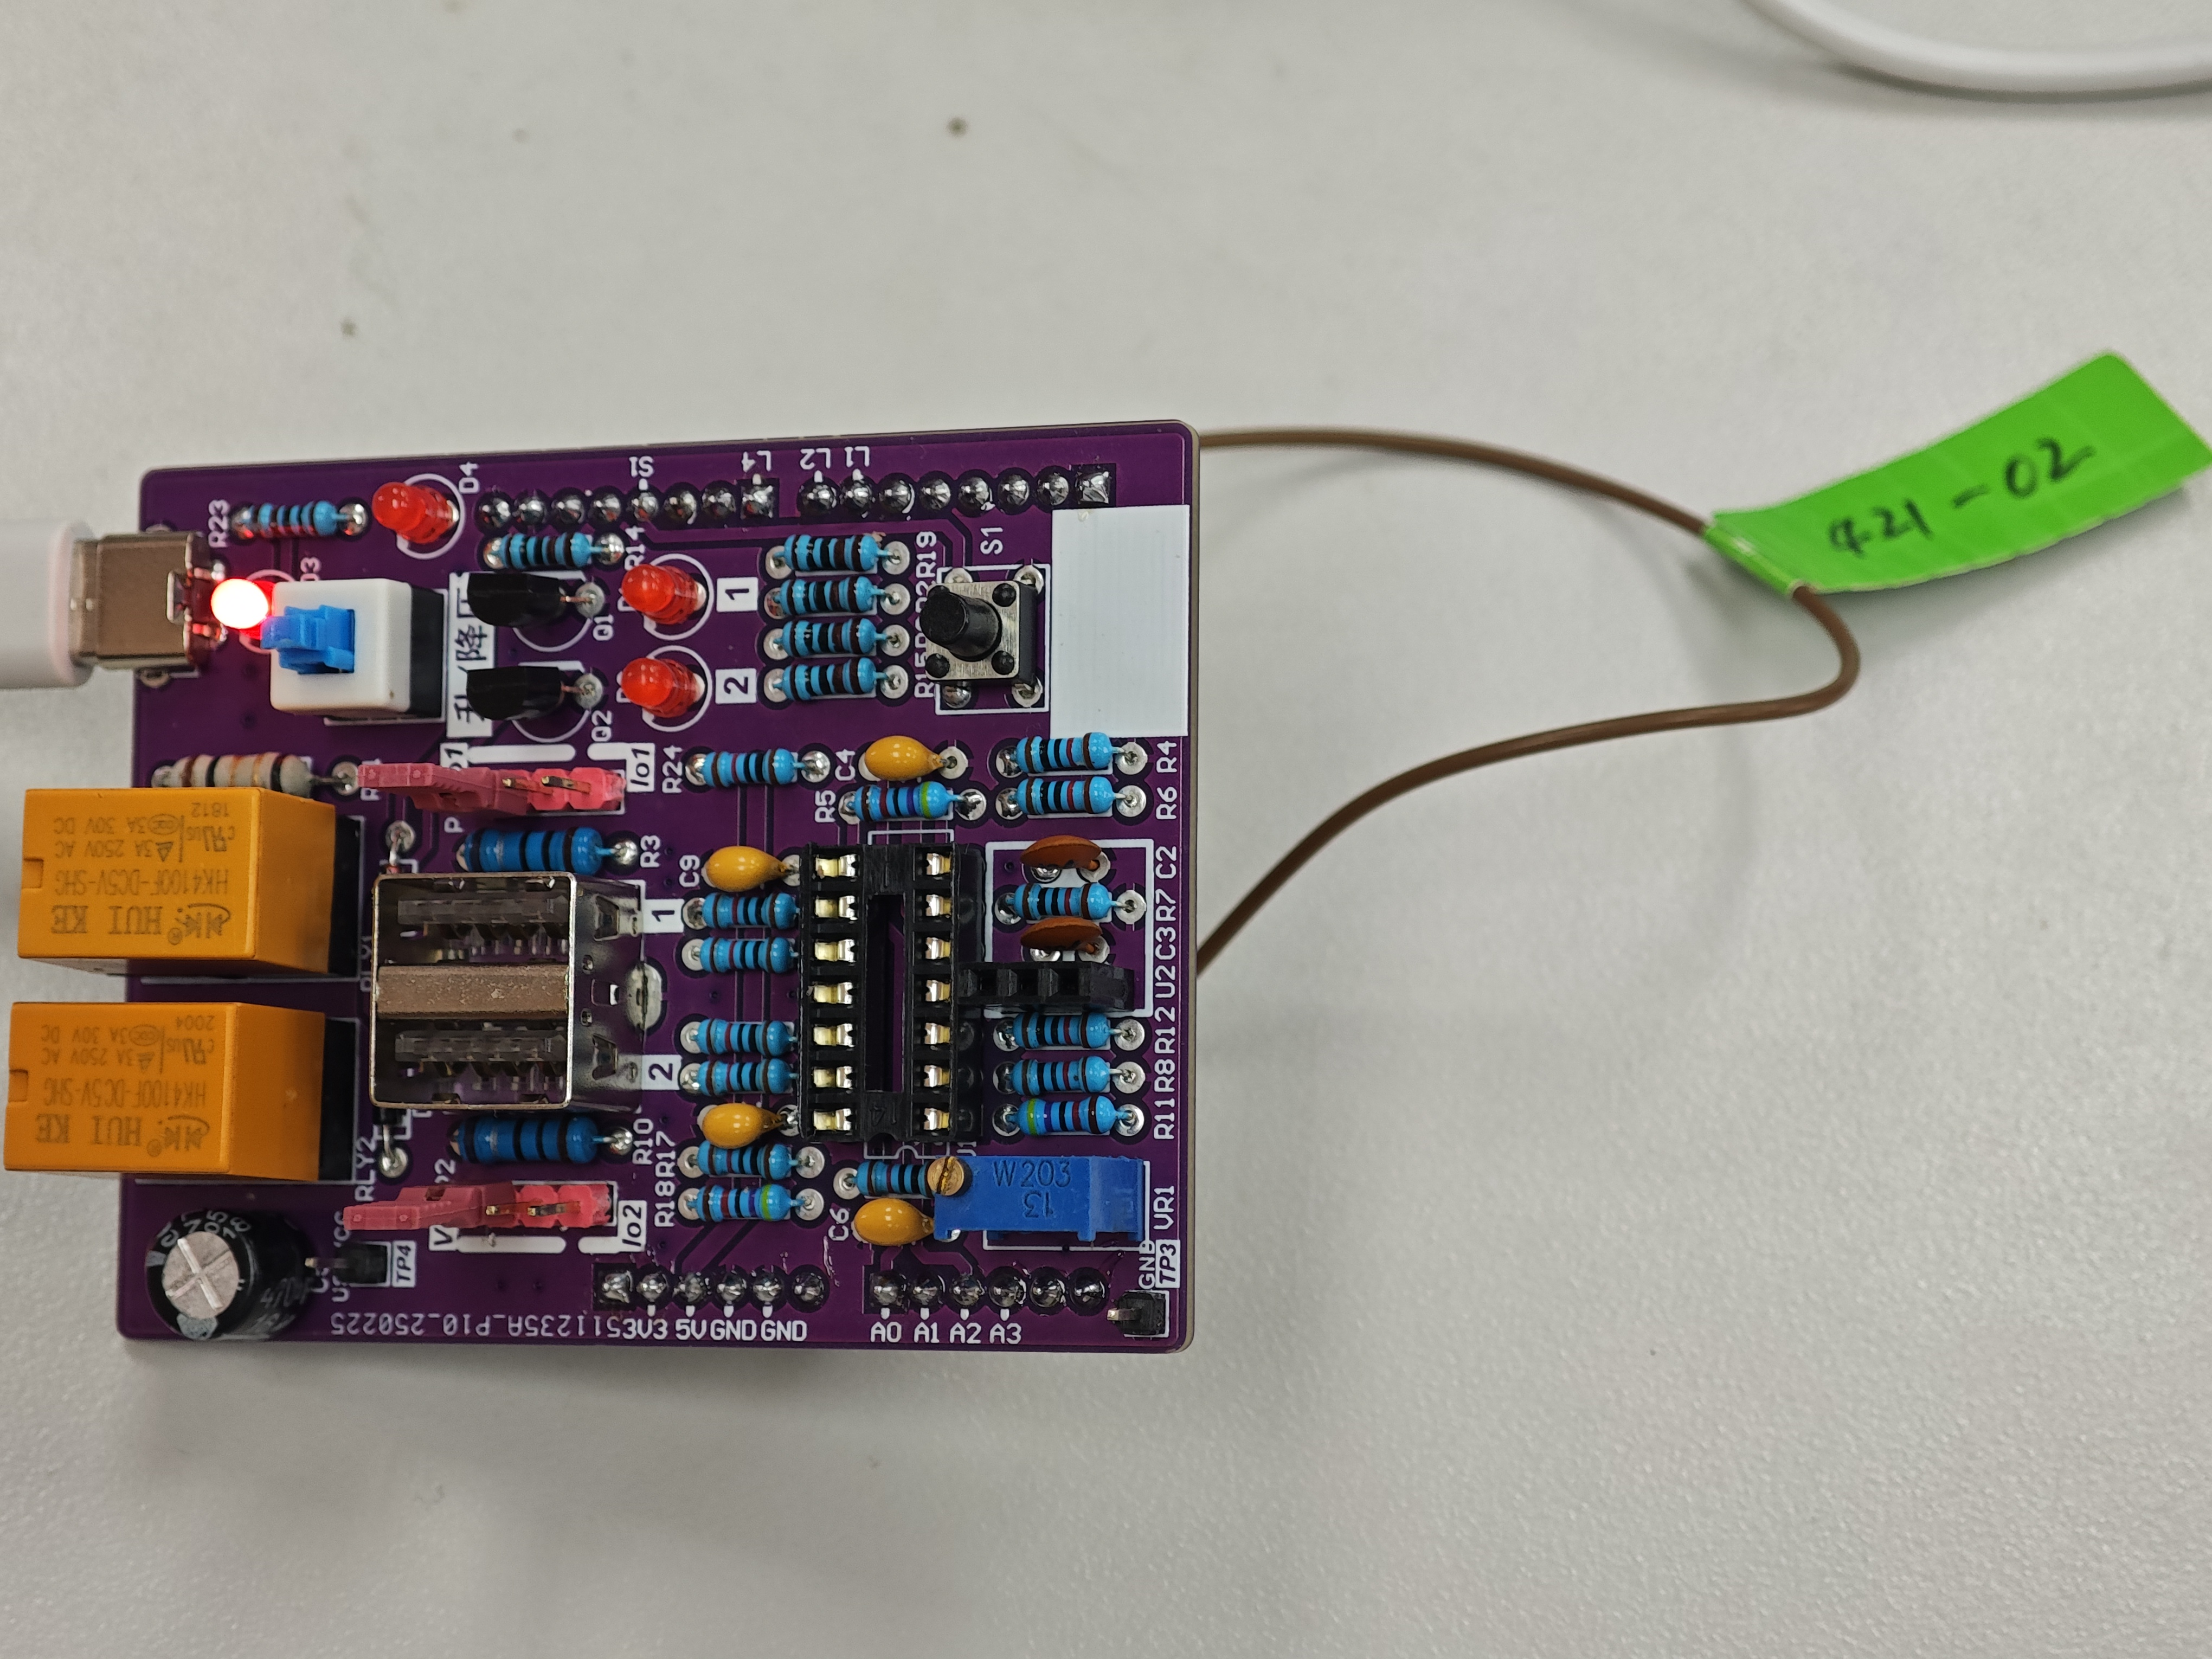
\includegraphics[width=.3\textwidth]{./figures/插座/usb1断电.jpg}
  \caption{L1,继电器RLY1测试}
\end{figure}
\begin{figure}[H]
  \centering
  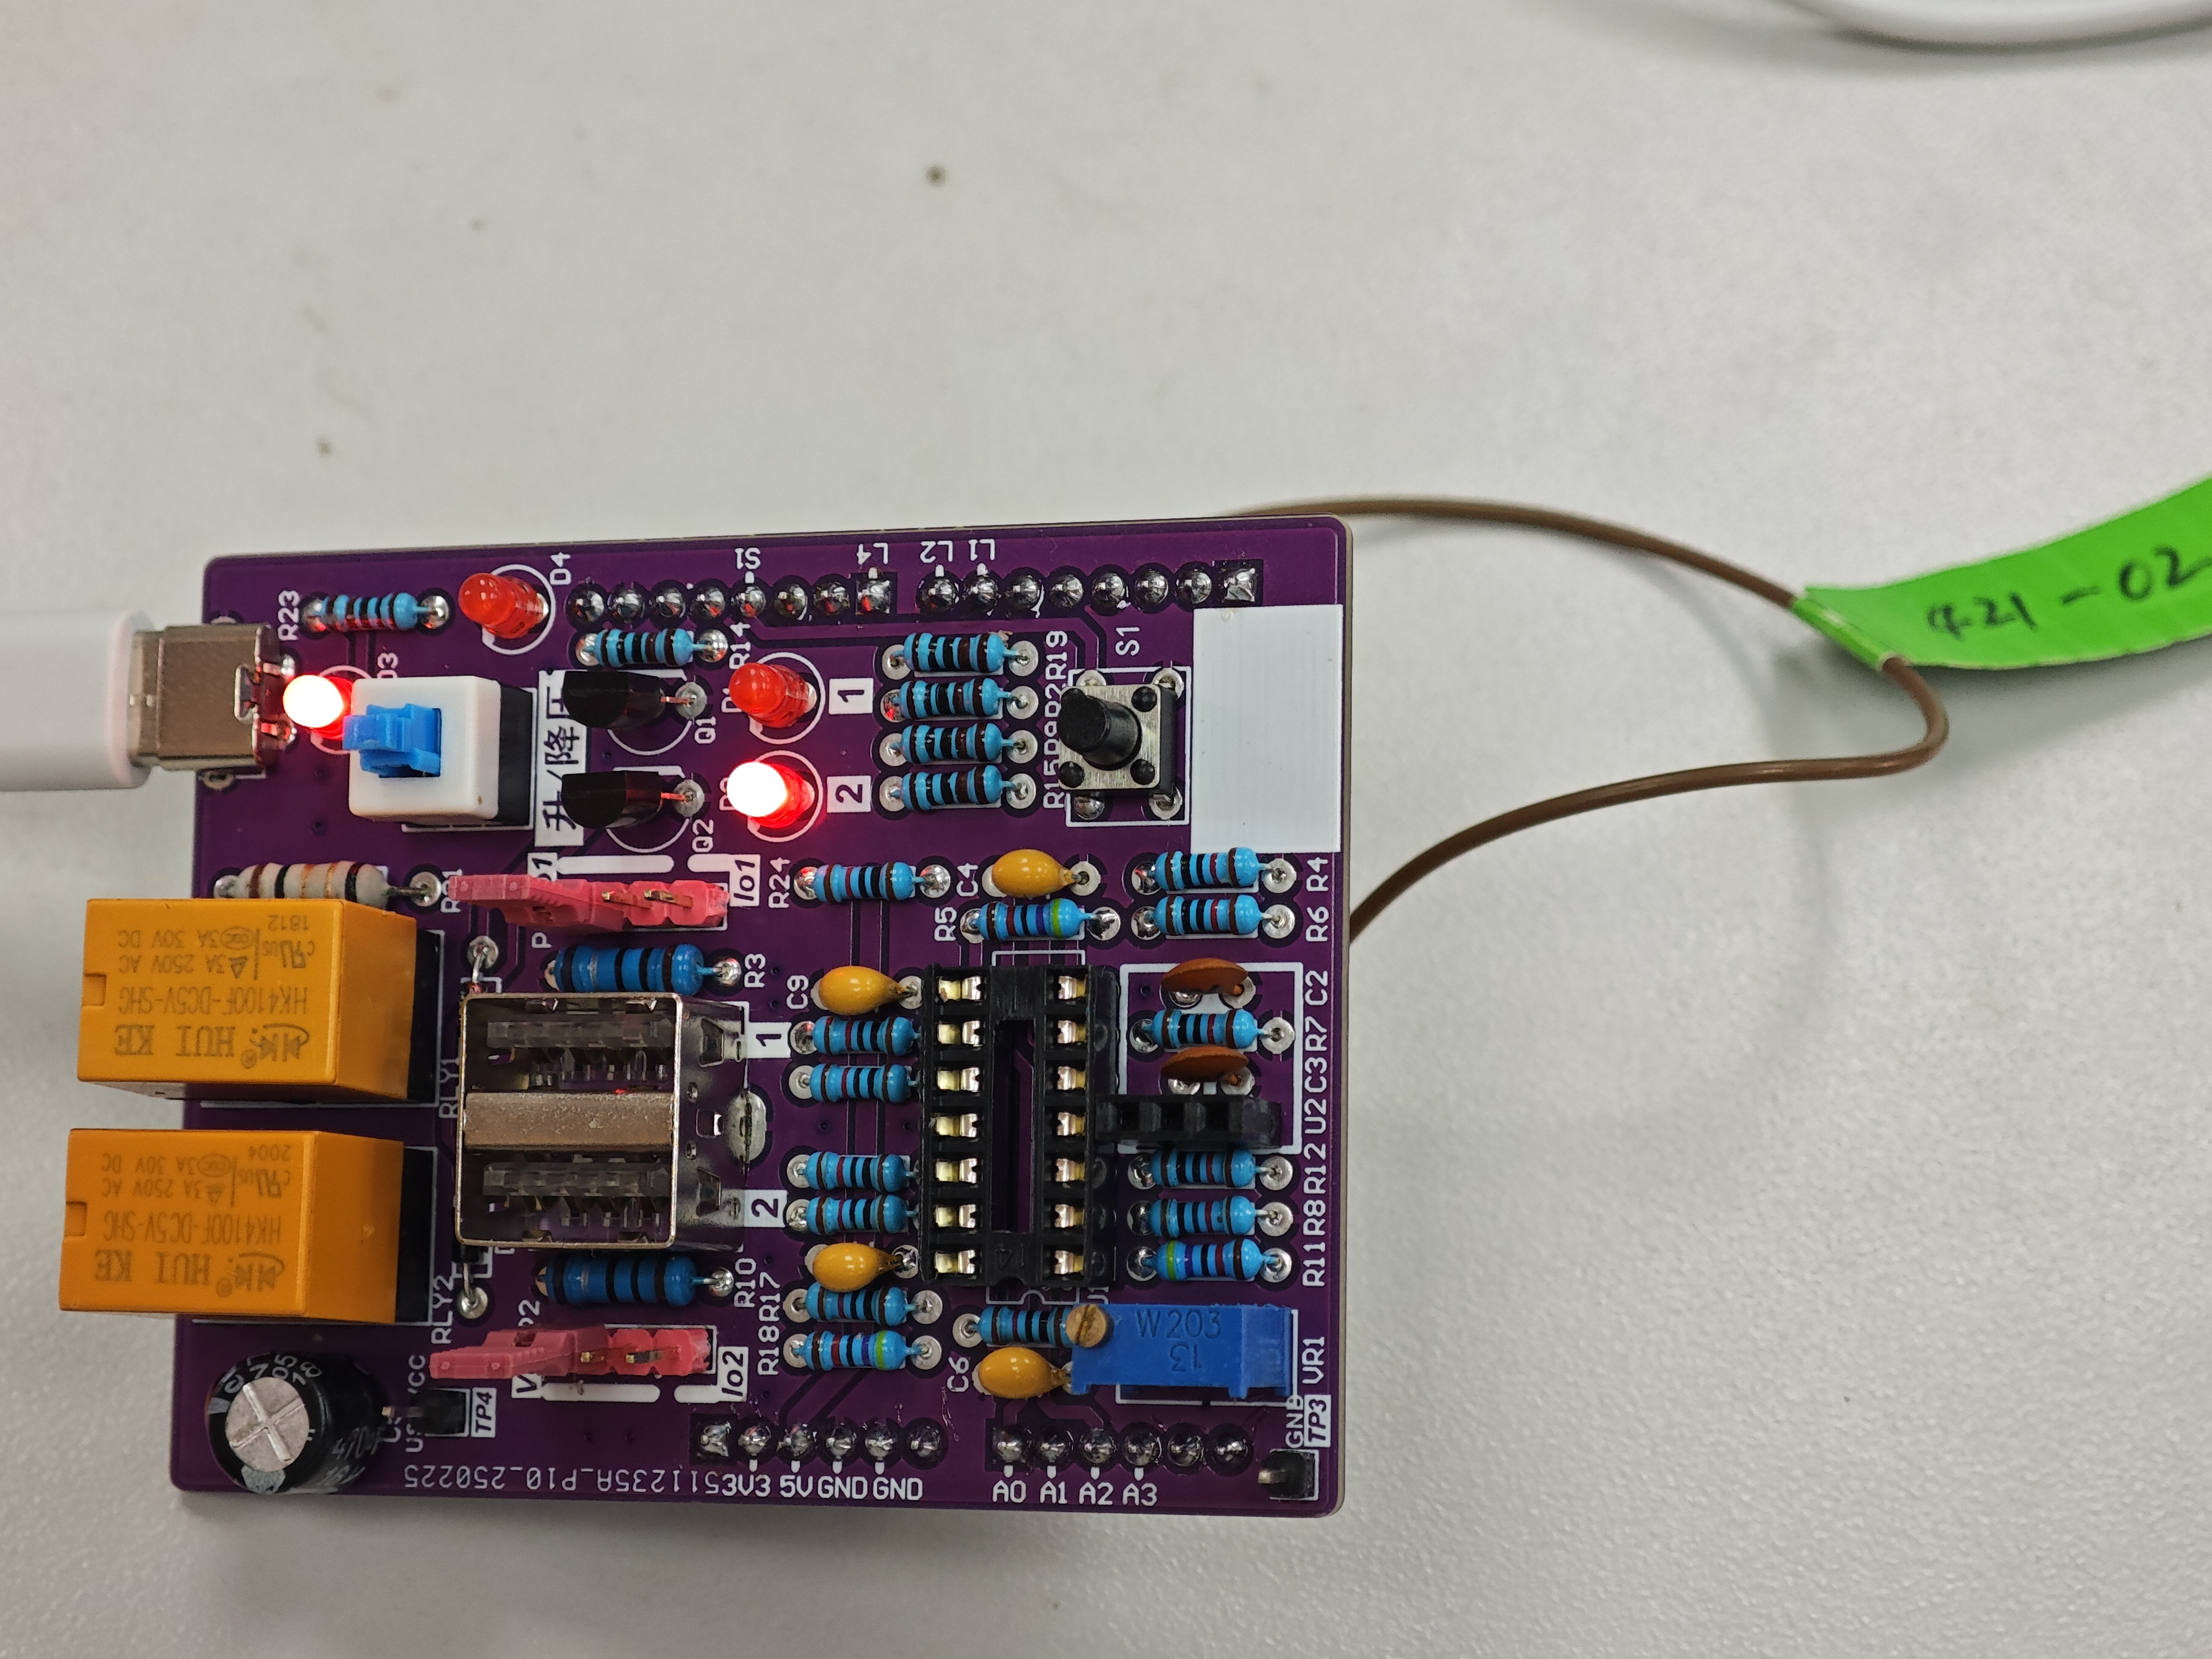
\includegraphics[width=.3\textwidth]{./figures/插座/usb2通电.jpg}
  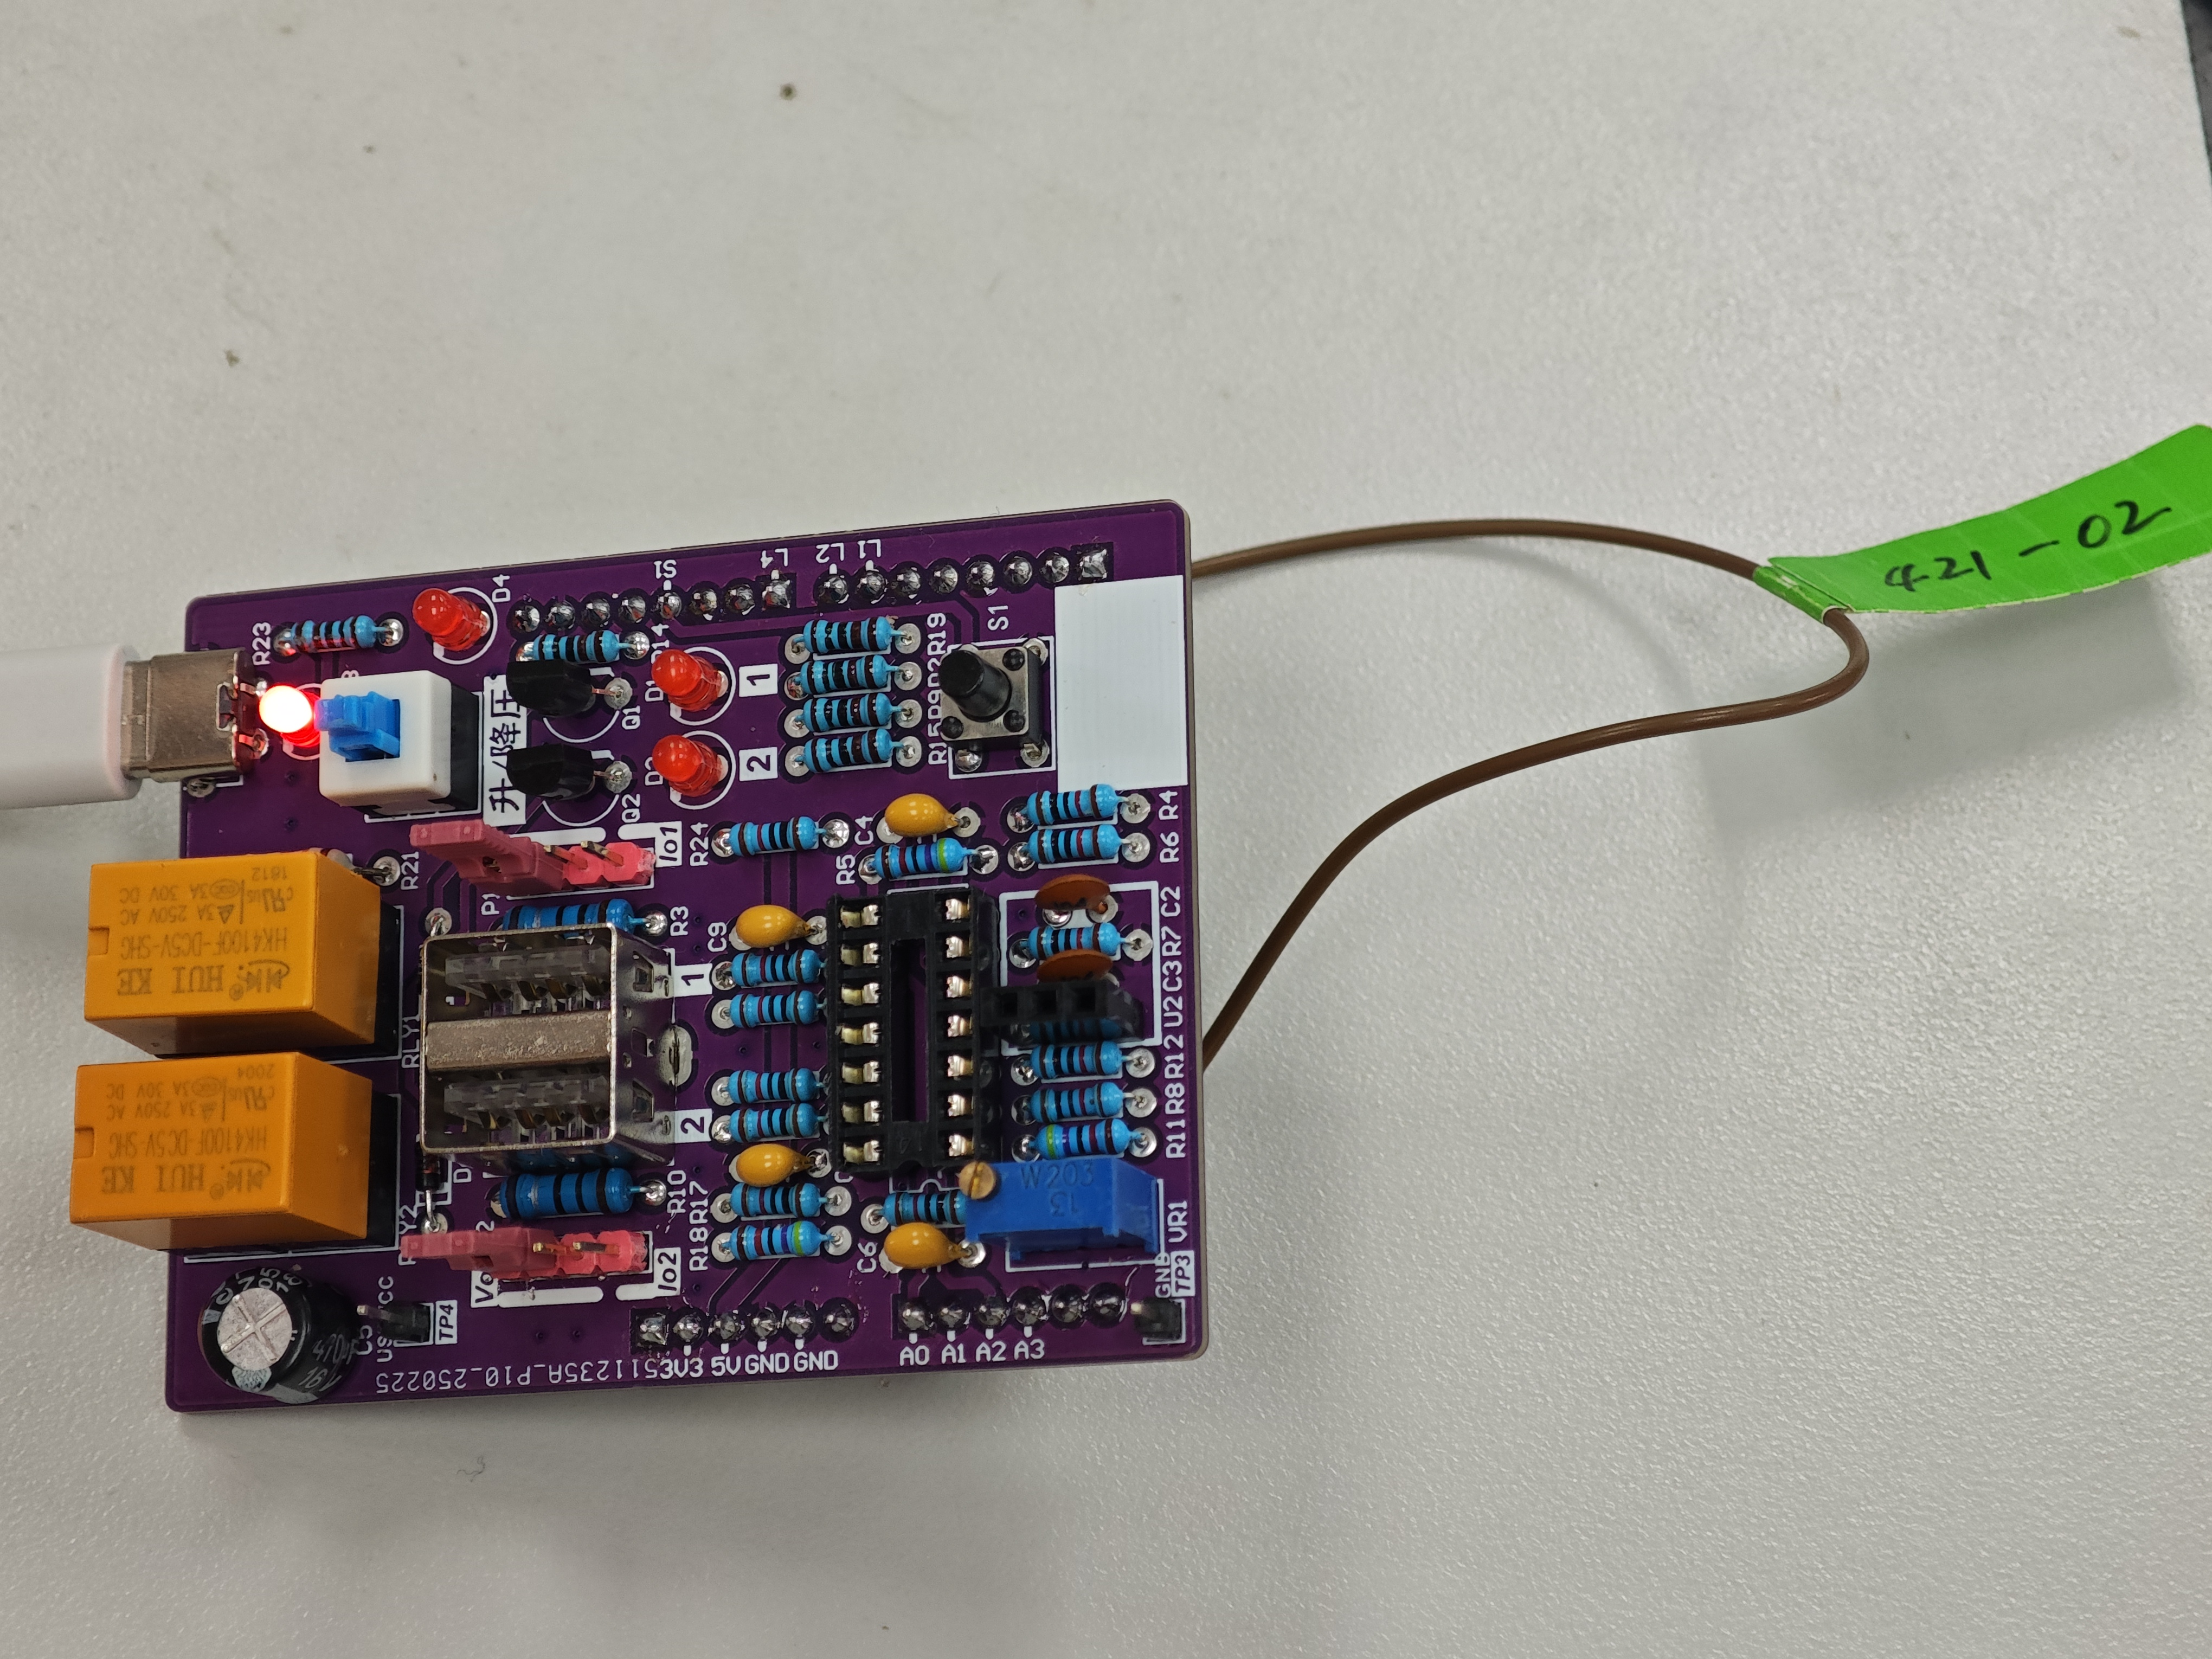
\includegraphics[width=.3\textwidth]{./figures/插座/usb2断电.jpg}
  \caption{L2,继电器RLY2测试}
\end{figure}
\subsection{指示灯测试}
\begin{table}[H]
\centering
\caption{指示灯测试结果}
\begin{tabular}{L{.4\textwidth}L{.4\textwidth}}
\toprule
检测项目  & 检测结果 \\
\midrule
电路上电,以杜邦线连接标注L4处至标注5V,观察到的现象:  & D4\underline{亮}。这里通过标注4所施加的5V电压,就是后续系统能通过软件输出的二进制控制信号``1''。 \\
电路上电,以杜邦线连接标注L4处至标注GND,观察到的现象:  & D4\underline{灭}。这里通过标注4所施加的0V电压,就是后续系统能通过软件输出的二进制控制信号``0''。 \\
\bottomrule
\end{tabular}
\end{table}
\begin{figure}[H]
\centering
 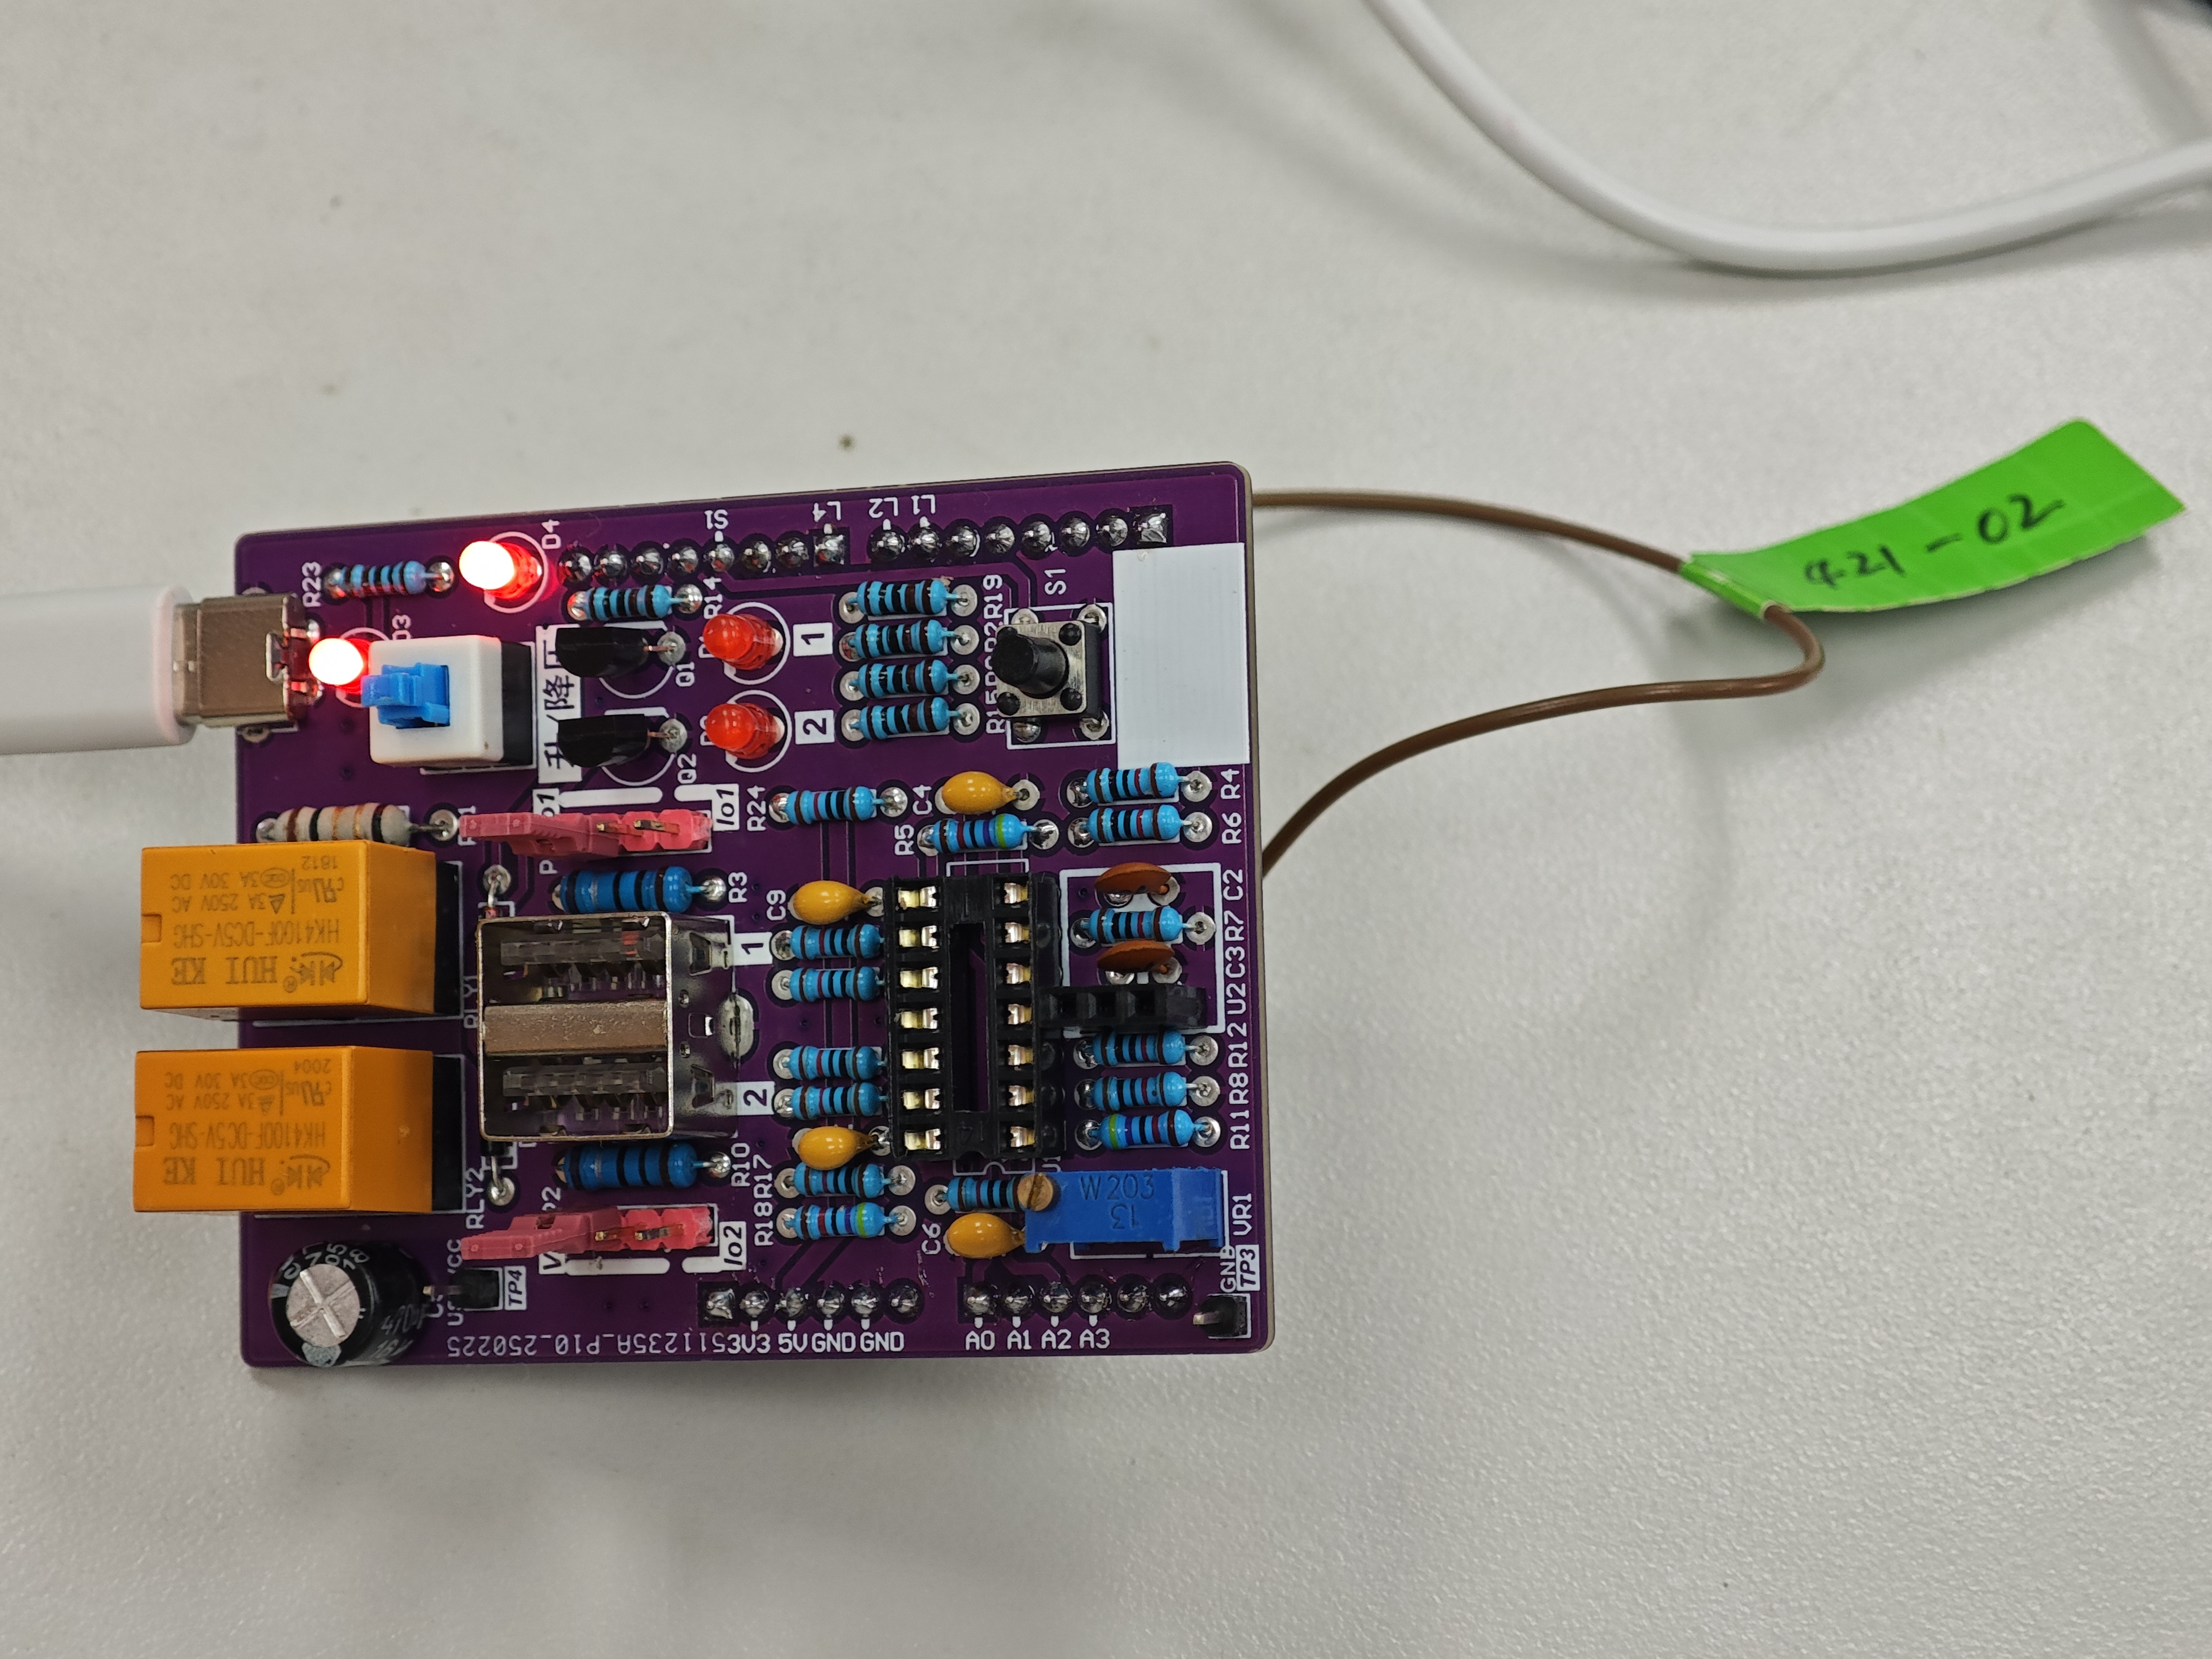
\includegraphics[width=.5\textwidth]{./figures/插座/控制D4.jpg}
 \caption{控制L4亮起}
\end{figure}
\subsection{集成电路芯片的供电检测}
\begin{table}[H]
    \centering
    \caption{集成电路芯片的供电检测结果}
    \begin{tabular}{L{.6\textwidth}C{.2\textwidth}}
    \toprule
    检测项目  & 检测结果 \\
    \midrule
    LM324AN 的电源电压(V): & 5.092V \\
    LM35DZ 的电源电压(V): &  5.103V \\
    \bottomrule
    \end{tabular}
    \end{table}
    \begin{figure}[H]
        \centering
         \includegraphics[width=.3\textwidth]{./figures/插座/集成电路供电.jpg}
         \hspace{5em}
         \includegraphics[width=.3\textwidth]{./figures/插座/温度传感器供电.jpg}
         \caption{测量集成电路供电}
        \end{figure}